
	\subsection{Когомологии циклической группы}

	Пусть $0 \to A \xrightarrow{i} B \xrightarrow{j} C \to 0$~--- короткая точная последовательность коэффициентов. Она индуцирует длинную точную последовательность когомологий

	\[
		0 \to A^G \to B^G \to C^G \xrightarrow{\delta} H^1(G, A) \to H^1(G, B) \to H^1(G, C) \xrightarrow{\delta} \ldots 
	\]

	Вспомним, как устроен связывающий гомоморфизм в маленьких размерностях. Возьмём $c \in C^G$, так как $j$~--- эпиморфизм, $\exists b\colon j(b) = c$. Тогда 
	\[
		j(gb - b) = gc - c = 0, \text{ так как } c \in C^G.
	\]
	Так как $\ker{j} = \Im{i}$, это означает, что $gb - b = i(a)$ для некоторого $a \in A$. Соответственно, мы можем определить функцию 
	\[
		\varphi\colon G \to A, \quad g \mapsto a, \text{ где } a\colon gb - b = i(a).
	\]


	Так как $i$~---мономорфизм, при фиксированном $b$ элемент $a$ определён однозначно. Теперь заметим, что  
	\[
		\begin{cases} g_1 b - b = i(a_1) \\ g_2 b - b = i(a_2)  \end{cases} \implies g_1 g_2 b - b = g_1(g_2 b - b) + (g_1 b - b) = g_1 i(a_2) + i(a_1) = i(g_1 a_2 + a_1).
	\]
	Таким образом, мы получили, что $\varphi(g_1g_2) = g_1 \varphi(g_2) + \varphi(g_1)$, то есть $\varphi$~--- 1-коцикл. 

	Значит, у нас есть отображение $C^{G} \to Z^{1}(G, A)$, определённое как $c \mapsto \varphi$. Заметим, что если мы выберем другой прообраз $b'$ вместо $b$, коцикл $\varphi$ изменится на кограницу и класс когомологий от этого не изменится. Итого, связывающий гомоморфизм в нулевом члене имеет такой вид: 
	\[
		\delta \colon C^{G} \to H^{1}(G, A), \quad c \mapsto [\varphi]. 
	\]

	Приступим теперь к подсчету когомологий $G = C_n = \langle \sigma \rangle, \ \sigma^n = e$. 

	\begin{definition} 
		Положим $N = \sum_{g \in G} g \in \Z[G]$. \emph{Норменным отображением} мы будем называть отображение 
		\[
			N\colon \Z[G] \to \Z[G], \quad a \mapsto N \cdot a. 
		\]
	\end{definition}

	Для циклической группы у нас есть такая проективная резольвента: 
	\[
		\ldots \xrightarrow{\cdot (\sigma - 1)} \Z[G] \xrightarrow{\cdot N} \Z[G] \xrightarrow{\cdot (\sigma - 1)} \Z[G] \xrightarrow{\varepsilon} \Z \to 0,
 	\]
 	где $\varepsilon$~--- аугументация. Проверим точность: 
 	\begin{itemize}
 		\item Пусть $x = \sum_{i = 0}^{n - 1} a_i \sigma^{i}$, тогда если $\varepsilon(x) = 0$, то $\sum_{i = 0}^{n - 1} a_i = 0$, откуда 
 		\[
 			x  = \sum_{i = 0}^{n - 1} a_i \sigma^{i}  = \sum_{i = 0}^{n - 1} a_i \sigma^{i}  - \sum_{i = 0}^{n - 1} a_i = \sum_{i = 0} a_i(\sigma^i - 1),
 		\]
 		откуда $x \in (\sigma - 1) \Z[G]$. 

 		\item Теперь пусть $(\sigma - 1) \lr*{\sum_{i = 0}^{n - 1} a_i \sigma^{i}} = 0$, тогда 
 		\[
 			a_0 + a_1 \sigma + \ldots + a_{n - 1}\sigma^{n - 1} = a_0 \sigma + a_1 \sigma^2 + \ldots + a_{n - 2}\sigma^{n - 1} + a_{n - 1} 
 		\]
 		Приравнивая коэффициенты при базисных элементах мы получаем:
 		\[
 			a_1 = a_0, a_2 = a_2, \ldots \implies a_0 = a_1 = \ldots = a_{n - 1} = a,
 		\]
 		откуда $x = Na$. 
 	\end{itemize}

 	и, точность в остальных членах тоже проверяется. Тогда наш комплекс будет иметь вид 
 	\[
 		0 \to \Hom_{G}(\Z[G], A) \xrightarrow{\cdot (\sigma - 1)} \Hom_{G}(\Z[G], A) \xrightarrow{\cdot N} \Hom_{G}(\Z[G], A) \to \ldots 
 	\]
 	Теперь вспомним, что $\Hom_{G}(\Z[G], A) \cong A$ и наш комплекс выглядит немного адекватнее: 
 	\[
 		0 \to A \xrightarrow{\cdot (\sigma - 1)} A  \xrightarrow{\cdot N} A \xrightarrow{\cdot (\sigma - 1)} A \xrightarrow{\cdot N} \ldots,
 	\]
 	откуда видно, что мы доказали такую теорему  

 	\begin{theorem} 
 		Пусть $G$~--- циклическая группа порядка $n$, а $A \in G\text{-}\Mod$. Тогда 
 		\[
 			H^{0}(A, G) = A^G, \quad H^{2i + 1}(G, A) \cong \ker{N}/(\sigma - 1)A, \quad H^{2i}(G, A) \cong A^{G}/N A.
 		\]
 	\end{theorem}

 	\begin{remark}
 		Мы тут немножко замяли под ковёр, но впрочем очевидно, что для циклической группы $(\sigma - 1)x = 0 \Leftrightarrow x \in A^{G}$. 
 	\end{remark}

 	\begin{statement} 
 		Пусть $G$~--- конечная группа, $0 \to A \to B \to C$~--- короткая точная последовательность. Тогда следующая последовательность точна: 
 		\[
 			A^{G}/NA \to B^{G}/NB \to C^{G}/NC \xrightarrow{\delta} H^{1}(G, A) \to \ldots
 		\]
 	\end{statement}
 	\begin{proof}
 		Запишем сначала длинную точную последовательность когомологий: 
 		\[
		0 \to A^G \xrightarrow{i^*} B^G \xrightarrow{j^*} C^G \xrightarrow{\delta} H^1(G, A) \to H^1(G, B) \to H^1(G, C) \xrightarrow{\delta} \ldots 
		\]
		По точности $\forall c \in C \ \exists b \in B \colon c = j(b)$. Тогда $j(Nb) = Nc$, а так как $Nb \in B^G$, мы получаем, что $Nc \in \Im{j^*} \subset \ker{\delta}$. Отсюда мы имеем $NC \subset \Ker{\delta}$. В остальных членах точность очевидна.  

 	\end{proof}

 	\subsection{Гомологии групп}

 	Пусть $G$~--- группа, $\Z$ мы рассматриваем, как $G$-модуль с тривиальным действием. Рассмотрим проективную резольвенту 
 	\[
 		\ldots \to P_{2} \to P_{1} \to P_0 \to \Z \to 0. 
 	\]
 	Применим к ней функтор $\_ \otimes_{\Z[G]} A$, получим комплекс 
 	\[
 		\ldots \to P_1 \otimes_{\Z[G]} A \to P_0 \otimes_{\Z[G]} A \to 0.
 	\]

 	Тогда $H_{i}(G, A)$ мы определим, как группы гомологий этого комплекса. 

 	\begin{remark}
 		Нетрудно проверить, что группы гомологий не зависят от выбора резольвенты.  
 	\end{remark}

 	\begin{example}[Нулевые гомологии]
 		Так как тезнорное произведение $\_ \otimes_{\Z[G]} A $ точно справа, последовательность 
 		\[
 			P_1 \otimes_{\Z[G]} A \to P_0 \otimes_{\Z[G]} A \to \Z \otimes_{\Z[G]} A \to 0
 		\]
 		точна. Отсюда $\Im\lr*{P_1 \otimes A \to P_0 \otimes A} \cong \ker\lr*{P_0 \otimes A \to \Z \otimes_{\Z[G]} A }$. Соответственно, 
 		\[
 			H_{0}(G, A) \cong \Z \otimes_{\Z[G]} A.
 		\]

 		Пусть $P_0 = \Z[G], $ а отображение $\varepsilon\colon P_0 \twoheadrightarrow \Z$~--- аугументация. Тогда, как мы помним, $\ker{\varepsilon} = I = \langle g - 1 \ \vert \ g \in G \rangle$~--- аугументационный идеал. Соответственно, у нас есть вот такая короткая точная последовательность: 
 		\[
 			0 \to I \to \Z[G] \xrightarrow{\varepsilon} \Z \to 0.
  		\]
  		Домножим её тензорно на $A$ над $\Z[G]$, получим точную последовательность 
  		\[
  			I \otimes_{\Z[G]} A \to \Z[G] \otimes_{\Z[G]}  A \to \Z \otimes_{\Z[G]} A \to 0,
  		\]
  		а так как $\Z[G] \otimes_{\Z[G]} A \cong A$, мы имеем 
  		\[
  			I \otimes_{\Z[G]} A \to A \to \Z \otimes_{\Z[G]} A \to 0,	
  		\]
  		а из точности этой последовательности мы заключаем, что 
  		\[
			\Ker\lr*{P_0 \otimes_{\Z[G}} A \to \Z \otimes_{\Z[G]} A \cong IA,
  		\]
  		откуда $H_{0}(G, A) \cong A/IA$.
 	\end{example}

 	Отметим, что для гомологий короткая точная последовательность коэффициентов $0 \to A \to B \to C \to 0$ также индуцирует длинную точную последовательность когомологий: 
 	\[
 		\ldots \to  H_{q}(G, A) \to H_{q}(G, B) \to H_{q}(G, C) \xrightarrow{\delta} H_{q - 1}(G, A) \to \ldots.
 	\]

 	\begin{theorem} 
 		$H_{1}(G, \Z) \cong G^{ab} = G/[G, G]$. 
 	\end{theorem}

 	\begin{proof}
 		Рассмотрим короткую точную последовательность 
 		\[
 			0 \to I_G \to \Z[G] \xrightarrow{\varepsilon} \Z \to 0,
 		\]
 		напишем соотвествующую длинную точную последовательность гомологий: 
 		\[
 			\ldots \to H_1(G, \Z[G]) \to H_1(G, \Z) \to H_0(G, I_G) \to H_0(G, \Z[G]) \to H_0(G, \Z) \to \ldots
 		\]

 		\begin{itemize}
 			\item Покажем, что $H_{1}(G, \Z[G]) = 0$. Действительно, если мы напишем проективную резольвенту для $\Z$ и тезнорно умножим её на $\Z[G]$, то полученный комплекс будет точным со второго члена (так как проективные модули свободны как абелевы группы, а тензорное произведение на таких~--- точный функтор) и все его гомологии (кроме нулевых) будут нулевыми. 

 			\item $H_0(G, \Z[G]) \cong \Z$  и $H_0(G, \Z) = \Z$, причем стрелка между ними~--- изоморфизм. 

 		\end{itemize}

 		Значит, наша точная последовательность на самом деле имеет вид 
 		\[
 			0 \to \ldots H_1(G, \Z) \xrightarrow{\sim} H_0(G, I_G) \xrightarrow{\cdot 0} \Z \xrightarrow{\sim} \Z \to \ldots,
 		\]
 		откуда $H_1(G, \Z) \cong H_0(G, I_G)$. С другой стороны, мы вычисляли нулевые гомологии: 
 		\[
 			H_0(G, I_G) \cong I_G/I_G^2.
 		\]

 		Остаётся доказать, что $I_{G}/I_{G}^2 \cong G^{\mathrm{ab}}$. 

 		Действительно, рассмотрим отображение 
 		\[
 			\varphi\colon G \to I/I^2, \quad g \mapsto g - 1 \pmod{I^2}.
 		\]
 		Убедимся, что отображение корректно определено:
 		\[
 			gh g^{-1}h^{-1} - 1 = (gh - hg)g^{-1}h^{-1},
 		\]
 		но в то же время 
 		\[
 			gh - g - h + 1 = (g - 1)(h - 1) \in I_G^2, \quad hg - g - h - 1 = (h - 1)(g - 1) \in I_G^2,
 		\]
 		\[
 			gh - g - h + 1 - (hg - g - h - 1) = gh - hg.
 		\]

 		Теперь построим обратное отображение таким образом
 		\[
 			x = \sum_{g \in G} a_g \cdot g \in I_G, \quad \psi(x) = \prod_{g \in G} g^{a_g} \pmod{G, G}. 
 		\]
 		\[
 			\psi((g - 1)(h - 1)) = \psi(gh - g - h + 1) = gh \cdot g^{-1} \cdot h^{-1} \equiv 0 \pmod{[G, G]},
 		\]
 		то есть $I_G^2$ лежит в ядре. Кроме того, легко видеть, что $\psi \circ \varphi = \varphi \circ \psi = \id$.
 	\end{proof}

    Соотвественно, как и с индуцированными модулями, мы можем рассмотреть 
 	\[
	 	0 \to A'' \to A_{*} \to A \xrightarrow{\varphi} 0, \text{ где } A_* = \Z[G] \otimes_{Z} A,
	 \]
	 гомоморфизм $\varphi$ действует как $\sigma \otimes a \mapsto a$, а $A'' = \ker{\varphi}$. Соотвественно, рассуждением аналогичным рассуждению для коиндуцированных модулей мы получаем, что гомологии с коэффициентами в $A^*$ тривиальны. Как и в случае с коиндуцированными модулями, при помощи длинной точной последовательности пары мы можем делать сдвиг размерности. 

    Кроме того, отметим, что если группа $G$ конечна, то  $\Hom(\Z[G], X) \cong \Z[G] \otimes_{\Z} X$ как $G$-модули. Действительно, изоморфизм выглядит вот так: 
	 \[
	  	\varphi \mapsto \sum_{G} g \otimes \varphi(g)
	  \] 

	  Соответственно, индуцированный модуль также является и коиндуцированным (и, когомологии в нём также тривиальны). 

 	\subsection{Когомологии Тейта}

 	\begin{definition} 
 		Пусть $G$~--- группа, $A \in G\text{-}\Mod$. Введём группы \emph{когомологий Тейта} с коэффициентами в $G$-модуле $A$:
 		\[
 			\widehat{H}^{-1}(G, A) \eqdef \ker{N_{A}}/IA, \quad \widehat{H}^{-n}(G, A) \eqdef H_{n - 1}(G, A) \text{ при } n \ge 2
 		\]
 		и, кроме того, 
 		\[
 			\widehat{H}^0(G, A) = A^G/N_A A, \quad \widehat{H}^n(G, A) \eqdef H^n(G, A) \text{ при }  n \ge 1.
 		\]
 	\end{definition}

 	Пусть $0 \to A \to B \to C$~--- короткая точная последовательность. Мы знаем, что тогда есть длинная точная последовательность гомологий и длинная точная последовательность когомологий. Утверждается, что если правильно (т.е. так, как в определении выше) подобрать нулевой и начальные члены, будет длинная точная последовательность для когомологий Тейта (бесконечная в две стороны!): 
 	\[
 	 	\ldots \to \widehat{H}^{-1}(G, A) \to \widehat{H}^{-1}(G, B) \to \widehat{H}^{-1}(G, C) \to \widehat{H}^{0}(G, A) \to \widehat{H}^{0}(G, B) \to \widehat{H}^{0}(G, C) \to \widehat{H}^{1}(G, A) \to \ldots
 	 \] 

 	 Соответственно, точность в отрицательном и в положительном куске мы знаем. Проверим точность на стыках. 

 	 \begin{itemize}
 	 	\item Построим сначала гомоморфизм $\Ker{N_C}/IC \to A^G/N_A A$. Рассмотрим диаграмму: 
 	 	\begin{center}
 	 		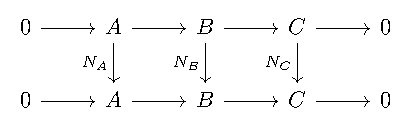
\includegraphics{lectures/6/pictures/cd_7.pdf}
 	 	\end{center}

 	 	Возьмём $c \in \Ker{N_C}$. У него есть какой-то прообраз при горизонтальном отображении, назовём его $b$ и рассмотрим $N_{B}b$. В силу коммутативности диаграммы, направо он уйдёт в ноль (так как $c \in \Ker{N_C}$), а значит, $N_{B}b$ лежит в образе стрелки  $f\colon A \to B$ в нижней части диаграммы. Тогда возьмём какой-то его прообраз $a$ (он определён однозначно, так как $f\colon A \to B$ инъективна). 

 	 	\item Покажем, что это построение корректно. $a \in A^{G}$, так как $N_B b \in B^G$. Если же мы выберем $b'$ вместо $b$, как прообраз, то $N_Bb - N_B b'$. Тогда $f^{-1}(N_Bb - N_B b') \in N_A A$. 

 	 	\item Покажем, что $IC$ попадает в 0 при отображении в $A^G/N_A A$. Проверим это для образующих аугументационного идеала, пусть $c = c' (g - 1) \in IC$, тогда $b = b' (g - 1)$, но тогда 
 	 	\[
 	 	 	N_B b = \lr*{\sum_{\sigma \in G} \sigma} b' (g - 1) = b'\lr*{ \sum_{\sigma \in G} \sigma g - \sum_{\sigma \in G} \sigma } = 0,
 	 	 \] 
 	 	 так как домножение на элемент группы это биекция. Точность проверяется как и обычно, технически. 
 	 \end{itemize}

    \noindent\bf{Тривиальность когомологий Тейта для индуцированного модуля} 

 	 Пусть $G$~--- конечная, группа $A_* \cong \Z[G] \otimes_{\Z} X$, где $X$~--- абелева группа (т.е. $A_*$~--- индуцированный модуль). Покажем, что 
 	 \[
 	 	H^{q}(G, A) = 0 \quad \forall q \in \Z.
 	 \]

 	 Для $q > 0$ мы это видели в замечании после определения индуцированного модуля. Рассмотрим теперь $q = 0$. Любой элемент $a \in A_*$ мы можем записать в виде 
 	 \[
 	 		a = \sum_{g} g \otimes x_{g}, \quad x_g \in X.
 	 \]
 	 Если $g'a = a$, то 
 	 \[
 	 	\sum_{g} (g' g \otimes x_g) = \sum_{g} g \otimes x_{g},
 	 \]
 	 в частности, $g' \otimes x_{g'} = g' \otimes x_{e}$, откуда $x_{g'} = x_{e}$. Соответственно, если $a \in A_*^G$, то $x_{g} = x_{e} \ \forall g \in G$ и отсюда 
 	 \[
 	 	a = \lr*{\sum_{g \in G} g} \otimes x_{e} = N\lr*{ e \otimes x_{e} } \implies a \in N_{G}A_*.
 	 \]
 	 Значит, $\widehat{H}^0(G, A_*) = A_*^G/NA_* = 0$. 

 	 Теперь пусть $q < -1$. Пусть $a \in \Ker{N}$, то есть 
 	 \[
 	 	N_G(\sum_{g} g \otimes x_{g}) = 0 \implies \sum_{g} x_{g} = 0 \implies \sum_{g} (g \otimes x_g) = \sum_{g} ((g - 1) \otimes x_g) \in I_G A_*,
 	 \]
 	 то есть $H^{-1}(G, A_*) = \Ker{N}/I_G A_* = 0$. 

 	 Пусть теперь $r < -1$. Возьмём для абелевой группы $X$ свободную резольвенту длины 2\footnote{достаточно накрыть свободной и взять ядро}: 
 	 \[
 	 	0 \to X_1 \to X_0 \to X \to 0.
 	 \]
 	 Тезнорно домножим эту последовательность на $\Z[G]$ (так как модули свободны, последовательность останется точной), получим последовательность 
 	 \[
 	 	 0 \to A_1 \to A_0 \to A_* \to 0
 	 \]

 	 Так как $A_1, A_0$~--- свободные $\Z[G]$-модули, 
 	 \[
 	 	H^{q}(G, A_1) = H^{q}(G, A_0) = 0 \quad \forall q < -1.
 	 \]
 	 А так как они индуцированные, $\forall q \ge -1$ 
 	 \[
 	 	H^{q}(G, A_1) = H^{q}(G, A_0) = 0.
 	 \]
 	 Таким образом, мы всё доказали. 


    \subsection{Периодичность когомологий Тейта для циклической группы}

 	 Так как далее мы будем часто сталкиватся с циклическими группами (в целях теории Галуа), полезно понимать, какие же у них когомологии Тейта. 

 	 \begin{theorem} 
 	 	Пусть $G$~--- циклическая группа конечного порядка, $A \in G\text{-}\Mod$. Тогда выбор образующей в $G$ задаёт изоморфизм 
 	 	\[
 	 		\widehat{H}^{q}(G, A) \cong \widehat{H}^{q + 2}(G, A) \quad \forall q \in \Z.
 	 	\]
 	 \end{theorem}
 	 \begin{proof}
 	 	Пусть $G = \langle \sigma \rangle$. Тогда имеется следующая короткая точная последовательность: 

 	 	\begin{center}
 	 		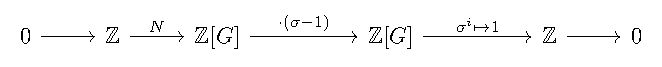
\includegraphics{lectures/6/pictures/cd_49.pdf}
 	 	\end{center}

 	 	Так как все члены последовательности, а также, аугументационный идеал $I_{G} = \Ker\lr*{\Z[G] \to \Z} $ свободны, как абелевы группы,  после тензорного умножения на $A$ последователньость останется точной: 

 	 	\begin{center}
 	 		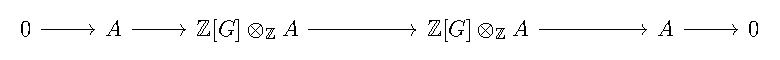
\includegraphics{lectures/6/pictures/cd_50.pdf}
 	 	\end{center}

 	 	Она, в свою очередь, разваливается в две короткие точные последовательности: 
 	 	\[
 	 		0 \to A \to \Z[G] \otimes_{\Z} A \to N_1 \to 0
 	 	\]
 	 	\[
 	 		0 \to N_1 \to \Z[G] \otimes_{\Z} A \to A \to 0.
 	 	\]
 	 	Записывая длинную точную последовательность пары мы для каждой из них, мы получаем, что 
 	 	\[
 	 		H^{q}(G, A) \cong H^{q + 1}(G, N_2) \cong H^{q + 2}(G, A),  
 	 	\]
 	 	что и даёт нам нужный факт. 
 	 \end{proof}


 	 \begin{remark}
 	 	Отметим, что это явление мы уже наблюдали для когомологий, но там была стандартная теория, а тут теория Тейта (и это существенно)!
 	 \end{remark}



   

 	 

